\documentclass[10pt]{beamer}
\setbeamertemplate{section in toc}[sections numbered]
\setbeamertemplate{subsection in toc}[subsections numbered]
%\setbeamertemplate{section in toc}[ball unnumbered]
%\setbeamertemplate{subsection in toc}[ball unnumbered]
\usetheme{Berlin} 
%\setbeamertemplate{footline}[frame number]

\usepackage{minted}
\usepackage{epsfig, amsfonts, amsbsy, amsmath}
\usepackage{hyperref}
\usepackage{algorithm2e}

\setbeamertemplate{blocks}[rounded][shadow=true]
\addtobeamertemplate{block begin}{\pgfsetfillopacity{0.8}}{\pgfsetfillopacity{1}}
\setbeamercolor*{block title example}{fg=blue!50,
bg=blue!15}
\setbeamercolor*{block body example}{fg= blue,
bg= blue!5}

\begin{document}
%\frame{\titlepage}
\author[Ryan Rubenzahl]{\begin{tabular}{c} 
	Ryan Rubenzahl \\
    \href{mailto:rrubenza@caltech.edu}{rrubenza@caltech.edu} \\ 
\end{tabular}}

%\date[\today]{\today}
\date[July 27, 2020]{July 27, 2020}
\title[Learning \LaTeX \hspace{.81\textwidth} \insertframenumber/\inserttotalframenumber]{{\Large Learning \LaTeX}}
\institute[Intro to Astronomy 2020]{Intro to Astronomy 2020}

% Turn off nav symbols
\beamertemplatenavigationsymbolsempty

% Abbreviated itemize environment
\def \bi {\begin{itemize}\item}
\def \ei {\end{itemize}}

\frame{\titlepage}

% WARNING: This beamer presentation will likely not compile if you are compiling from a local TeX distribution - you will need to install the minted package to activate the syntax-highlighted code blocks. Minted also requires a Python package, pygmentize, to work. Installing this is annoying. Further, an extra command-line option must be used for the document to compile properly. Check 
% https://tex.stackexchange.com/questions/279214/pygmentize-not-working-properly-with-minted-package-in-texshop-on-os-x
% if you have issues installing it on Mac OS X.
% Alternatively, Overleaf has (basically) every LaTeX package available, so this should run fine there


%%%%%%%%%%%%%%%%%%%%%%%%%%%%%%%%%%%%%%%%%%%%%%%%%%%%%%%%%%%%%%%%%%%%%%%%%%%%%%%%%%%%%%%   S   L   I   D   E   %%%%%%%%%%%%%%%%%%%%%%%%%%
%%%%%%%%%%%%%%%%%%%%%%%%%%%%%%%%%%%%%%%%%%%%%%%%%%%%%%%%%%%%%
\AtBeginSection[]{
\begin{frame}
\frametitle{Outline}
\tableofcontents[currentsection]
\end{frame}
}

\section{What is \LaTeX? Why should I use it?}
\begin{frame}{What is \LaTeX? Why should I use it?}
	\bi LaTeX (Lay-TECH or Lah-TECH) is a typesetting software that is designed for producing scientific and mathematical documents of high typographical quality \ei
	\bi \LaTeX \, worries about formatting, you worry about content \ei
	\begin{center}
	
\includegraphics[width=0.35\textwidth]{./figures/latex-comic.jpeg}
	\hspace{25pt}
	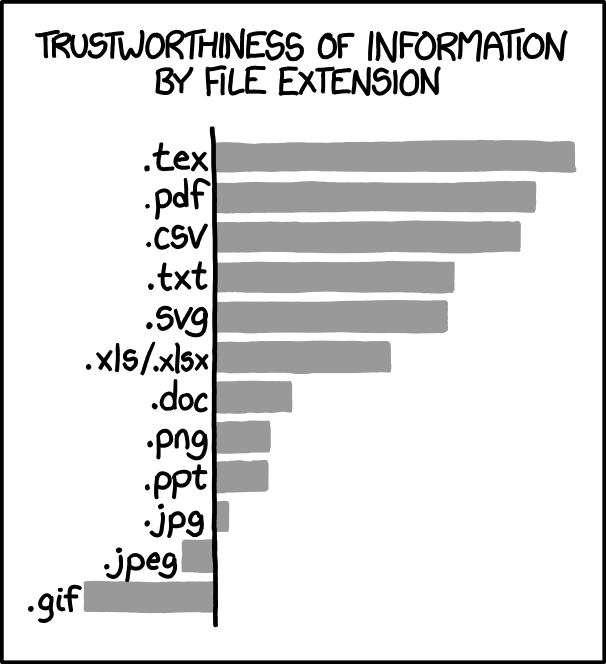
\includegraphics[width=0.35\textwidth]{./figures/file_extensions.png} % https://xkcd.com/1301/    (file extentions)
	\end{center}
\end{frame}

%%%%%%%%%%%%%%%%%%%%%%%%%%%%%%%%%%%%%%%%%%%%%%%%%%%%%%%%%%%%%%%%%%%%%%%%%%%%%%%%%%%%%%%   S   L   I   D   E   %%%%%%%%%%%%%%%%%%%%%%%%%%
%%%%%%%%%%%%%%%%%%%%%%%%%%%%%%%%%%%%%%%%%%%%%%%%%%%%%%%%%%%%%
\section{How can I get \LaTeX?}
\begin{frame}[fragile]{How can I get \LaTeX?}

	\bi So \LaTeX will make my papers look beautiful and make me more trustworthy. How can I harness this power? \ei
	\bi Either install a \alert{local \TeX \, distribution}, or use an \alert{online editor} \ei
	\bi \TeX \, distributions:
	\bi \href{http://www.tug.org/texlive/}{\underline{\TeX{} Live}} (GNU/Linux, Mac OS, Windows) \ei
	\bi \href{http://tug.org/mactex/}{\underline{Mac\TeX}} (Mac OS) \ei
	\bi \href{https://miktex.org/}{\underline{MiK\TeX}} (Windows) \ei \ei
	
	\bi May not include an \textit{editor}, e.g. Mac\TeX{} comes with \TeX Shop, a \LaTeX \, editor/previewer
	\bi Can always use your own favorite text editor (e.g. Vim), and compile from the command line via \ei \ei
	\begin{minted}{bash}
		pdflatex mydocument.tex
	\end{minted}
	\bi \textbf{Online editor:} \href{https://www.overleaf.com/}{\underline{Overleaf}} (Google docs for \LaTeX) \ei

\end{frame}
%%%%%%%%%%%%%%%%%%%%%%%%%%%%%%%%%%%%%%%%%%%%%%%%%%%%%%%%%%%%%%%%%%%%%%%%%%%%%%%%%%%%%%%   S   L   I   D   E   %%%%%%%%%%%%%%%%%%%%%%%%%%
%%%%%%%%%%%%%%%%%%%%%%%%%%%%%%%%%%%%%%%%%%%%%%%%%%%%%%%%%%%%%
\section{Learning \LaTeX\, / Getting started}
\begin{frame}{Learning \LaTeX\, / Getting Started}

\begin{minipage}{0.5\textwidth}
\bi The \href{https://www.overleaf.com/learn}{\underline{tutorials on Overleaf}} are fantastic for getting started \ei
\bi The \href{https://en.wikibooks.org/wiki/LaTeX/}{\underline{TeX wiki}} is another great resource/guide \ei
\bi Many great templates to try out on \href{https://www.overleaf.com/latex/templates/}{\underline{Overleaf}}
\bi For professional journal templates, check out: \href{https://journals.aps.org/revtex}{\underline{REVTeX}} (aps, aip, prl, etc.) \ei \ei
\bi For a full-length starter guide, check out \textit{\href{https://tobi.oetiker.ch/lshort/lshort-letter.pdf}{The Not So Short Introduction to \LaTeX}}\, \cite{notsoshort} \ei
\end{minipage}
\hfill
\begin{minipage}{.45\textwidth}

\includegraphics[width=\textwidth]{./figures/learnlatex.png} % Credit LaTeX memes for well typeset teens https://www.facebook.com/badness10000/
{\footnotesize \underline{Via \href{https://www.facebook.com/badness10000/}{\LaTeX\, memes for well typeset teens}}}

\end{minipage}
\end{frame}


\section{Help/Troubleshooting Resources}
\begin{frame}{Help/Troubleshooting Resources}

	\begin{center}
	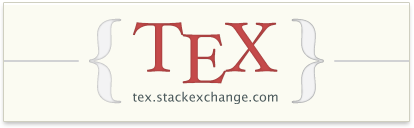
\includegraphics[width=0.5\textwidth]{./figures/texstackexchange.png}
	\end{center}

	\bi Unless you are literally a god, compiling your \LaTeX \, document will probably not be error-free every time
	\bi e.g. \texttt{Underfull \textbackslash hbox (badness 10000)} \ei \ei
	\bi Google is your friend, but your best friend is
	\bi \href{https://tex.stackexchange.com/}{\underline{TeX stack exchange}} \ei \ei
	\bi Forgot the command for that one symbol? Check out \href{http://detexify.kirelabs.org/classify.html}{\underline{Detexify}}
	\bi Lets you draw the symbol, and tells you the code for it \ei
	\bi If you have a Mac, you can download Detexify as an app! \ei \ei
	
\end{frame}
	
%%%%%%%%%%%%%%%%%%%%%%%%%%%%%%%%%%%%%%%%%%%%%%%%%%%%%%%%%%%%%%%%%%%%%%%%%%%%%%%%%%%%%%%   S   L   I   D   E   %%%%%%%%%%%%%%%%%%%%%%%%%%
%%%%%%%%%%%%%%%%%%%%%%%%%%%%%%%%%%%%%%%%%%%%%%%%%%%%%%%%%%%%%
\section{Making a Document}
\begin{frame}[fragile]{Basic Commands}
	\bi All command begin with a backslash `\textbackslash{}' and take one of two formats:
		\bi Command name consists \alert{only of letters}, terminated by a space/number/`non-letter' 
		\bi e.g. \mintinline{latex}{\LaTeX, \hfill, \newline} \ei \ei
		\bi Command name consists of a \alert{backslash and exactly one non-letter}
		\bi e.g. \mintinline{latex}{\,, \;, \{, \}}\ei \ei \ei
	\bi A command may also take parameters: \ei
	\begin{minted}{latex}
	\command[optional parameter]{parameter}
	\end{minted}
	\bi One may also \alert{define their own command}:
	\begin{minted}{latex}
	\newcommand{name}[num]{definition}
	\end{minted}
	\bi \texttt{num} = number of parameters, which are referred to in \texttt{definition} by \texttt{\#1}, \texttt{\#2}, etc. Command is called with \mintinline{latex}{\name} just like any other. \ei \ei
\end{frame}	

%%%%%%%%%%%%%%%%%%%%%%%%%%%%%%%%%%%%%%%%%%%%%%%%%%%%%%%%%%%%%%%%%%%%%%%%%%%%%%%%%%%%%%%   S   L   I   D   E   %%%%%%%%%%%%%%%%%%%%%%%%%%
%%%%%%%%%%%%%%%%%%%%%%%%%%%%%%%%%%%%%%%%%%%%%%%%%%%%%%%%%%%%%
\begin{frame}[fragile]{Making a Document: Setup}
	\bi \alert{Preamble}: section of code between \mintinline{latex}{\documentclass} and \mintinline{latex}{\begin{document}} \ei
	\bi Document Classes: Defined by \mintinline{latex}{\documentclass[options]{class}}
	\bi \texttt{options} specify the behavior of the document, e.g. font-size, paper-size, one/two column, etc. \ei
	\bi \texttt{class} specifies the type of document, e.g. article, beamer, report, book, etc. \ei \ei
	\bi The preamble is also where one can \alert{import packages} 
	\begin{minted}{latex}
	\usepackage[options]{package}
	\end{minted}
	\bi E.g. amsmath, amssymbol, hyperref, TikZ, physics, cancel, minted \ei \ei
	\bi The actual document is then started with a \mintinline{latex}{\begin{document}} and ended with \mintinline{latex}{\end{document}} \ei
\end{frame}	
%	
\begin{frame}[fragile]{Making a Document: Example}
	\begin{block}{Example: The Preamble}
	\begin{minted}[breaklines]{latex}
	\documentclass[11pt, letterpaper]{article}   	
	\usepackage[top=2.2cm, bottom=2cm, left=1cm, right=2cm]{geometry}                		
             		
	\usepackage{fancyhdr}

	\usepackage{physics}
	\usepackage{amssymb, amsmath}
	\usepackage{cancel}

	\begin{document}
	...
	\end{document}
	\end{minted}
	\end{block}
\end{frame}

%%%%%%%%%%%%%%%%%%%%%%%%%%%%%%%%%%%%%%%%%%%%%%%%%%%%%%%%%%%%%%%%%%%%%%%%%%%%%%%%%%%%%%%   S   L   I   D   E   %%%%%%%%%%%%%%%%%%%%%%%%%%
%%%%%%%%%%%%%%%%%%%%%%%%%%%%%%%%%%%%%%%%%%%%%%%%%%%%%%%%%%%%%

\begin{frame}[fragile]{Sections}
	\bi To define the start of a section, simply use the appropriate command: \ei
	\begin{minted}{latex}
	\section{...}, \subsection{...}, \subsubsection{...}
	\paragraph{...}, \subparagraph{...}
	\end{minted}
	\bi The section will be ``in effect'' until a new section command is encountered or the document ends
	\bi Only with \texttt{report} or \texttt{book} class: \mintinline{latex}{\chapter{...}} \ei \ei
	\bi Some special sections do not take an argument, e.g. \ei
	\begin{minted}{latex}
	\abstract, \appendix, \tableofcontents
	\end{minted}
	\bi Sections can be cross-referenced with the use of \alert{labelling} \ei
	\begin{block}{Example: Cross-referencing}
	\begin{minted}{latex}
	\section{Introduction\label{sec:intro}}
	Here is the intro, Section \ref{sec:intro}
	\end{minted}
	\end{block}
\end{frame}

%%%%%%%%%%%%%%%%%%%%%%%%%%%%%%%%%%%%%%%%%%%%%%%%%%%%%%%%%%%%%%%%%%%%%%%%%%%%%%%%%%%%%%%   S   L   I   D   E   %%%%%%%%%%%%%%%%%%%%%%%%%%
%%%%%%%%%%%%%%%%%%%%%%%%%%%%%%%%%%%%%%%%%%%%%%%%%%%%%%%%%%%%%

\begin{frame}[fragile]{Environments}
\bi A \LaTeX{} \alert{environment} is a way of grouping part of a document according to some formatting rules
\bi Environments may be nested so long as order is maintained \ei \ei
\bi Declared with \mintinline{latex}{\begin{environment}} and ended with \mintinline{latex}{\end{environment}}
\bi The main \mintinline{latex}{\begin{document}} and \mintinline{latex}{\end{document}} itself is an example of an environment \ei \ei
\bi Some common environments:
	\bi \texttt{itemize} for simple (bulleted) lists, \texttt{enumerate} for enumerated lists \ei
	\bi \texttt{tabular}, \texttt{table}, \texttt{figure}, \texttt{minipage}, \texttt{center}, \texttt{quote} \ei 
	\bi \texttt{equation}, \texttt{align} \ei
	\bi \texttt{frame} (Beamer) \ei \ei
\end{frame}

%%%%%%%%%%%%%%%%%%%%%%%%%%%%%%%%%%%%%%%%%%%%%%%%%%%%%%%%%%%%%%%%%%%%%%%%%%%%%%%%%%%%%%%   S   L   I   D   E   %%%%%%%%%%%%%%%%%%%%%%%%%%
%%%%%%%%%%%%%%%%%%%%%%%%%%%%%%%%%%%%%%%%%%%%%%%%%%%%%%%%%%%%%

\begin{frame}[fragile]{Writing Mathematical Equations}
	\bi For mathematical typesetting, \alert{use \AmS-\LaTeX} \ei
	\begin{minted}{latex}
	\usepackage{amsmath, amssymb, amsfonts, amsbsy}
	\end{minted}
	\bi See \href{https://oeis.org/wiki/List_of_LaTeX_mathematical_symbols}{\underline{list of Greek letters and mathematical symbols}} \ei
	\bi Several different ``math-mode'' environments: \ei
	%% Inline
	\begin{minipage}{0.45\textwidth}
	\begin{block}{Inline math-mode (source)}
	\centering
\begin{minted}{latex}
For $x \ll 1$ we can...
\end{minted}
	\end{block}
	\end{minipage}
	\hfill
	\begin{minipage}{0.45\textwidth}
	\begin{block}{Inline math-mode (output)}
	For $x \ll 1$ we can...
	\end{block}
	\end{minipage}
	%% equation
	\begin{minipage}{0.45\textwidth}
	\begin{block}{Equation math-mode (source)}
	\centering
\begin{minted}{latex}
The equation of motion
\begin{equation}
m \ddot{x} + kx = 0
\end{equation}
describes a harmonic...
\end{minted}
	\end{block}
	\end{minipage}
	\hfill
	\begin{minipage}{0.45\textwidth}
	\begin{block}{Equation math-mode (output)}
	The equation of motion
\begin{equation}
m \ddot{x} + kx = 0
\end{equation}
	describes a harmonic oscillator.
	\end{block}
	\end{minipage}
\end{frame}
% MORE EQUATIONS
\begin{frame}[fragile]{Writing Mathematical Equations}
\bi More math environments: \ei
%% unnumbered \[ \]
	\begin{minipage}{0.45\textwidth}
	\begin{block}{Unnumbered Eq. (source)}
	\centering
\begin{minted}{latex}
The Pythagorean Theorem, 
\[ a^2 + b^2 = c^2 \]
\end{minted}
	\end{block}
	\end{minipage}
	\hfill
	\begin{minipage}{0.45\textwidth}
	\begin{block}{Unnumbered Eq. (output)}
	The Pythagorean Theorem, 
	\[ a^2 + b^2 = c^2 \]
	\end{block}
	\end{minipage}
	% ALIGN W/ BOXED
	\begin{minipage}{0.45\textwidth}
	\begin{block}{Multiline Eq. (source)}
	\centering
\begin{minted}{latex}
The net force is
\begin{align*}
F_{net} &= \sum_i F_i \\
	&= F - F_f \\
	&= m a
\end{align*}
\end{minted}
	\end{block}
	\end{minipage}
	\hfill
	\begin{minipage}{0.45\textwidth}
	\begin{block}{Multiline Eq. (output)}
	The net force is
	\begin{align*}
	F_{net} &= \sum_i F_i \\
		&= F - F_f \\
		&= m a
	\end{align*}
	\end{block}
	\end{minipage}
\end{frame}

%%%%%%%%%%%%%%%%%%%%%%%%%%%%%%%%%%%%%%%%%%%%%%%%%%%%%%%%%%%%%%%%%%%%%%%%%%%%%%%%%%%%%%%   S   L   I   D   E   %%%%%%%%%%%%%%%%%%%%%%%%%%
%%%%%%%%%%%%%%%%%%%%%%%%%%%%%%%%%%%%%%%%%%%%%%%%%%%%%%%%%%%%%

\begin{frame}[fragile]{Figures}
	\begin{block}{Example: Figure}
\begin{minted}{latex}
\begin{figure}
\centering
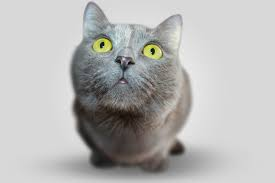
\includegraphics[width=0.2\textwidth]{./Figures/cat.png}
\caption{An image of a cat.}
\label{img:cat image}
\end{figure}
	\end{minted}
	\end{block}
	\begin{block}{Example: Figure}
	\begin{figure}
	\centering
	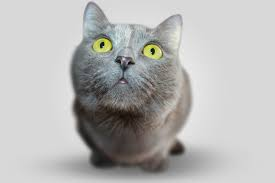
\includegraphics[width=0.2\textwidth]{./Figures/cat.png}
	\caption{An image of a cat.}
	\label{img:cat image}
	\end{figure}
	\end{block}
\end{frame}
%%%%%%
\begin{frame}[fragile]{Tables}
\begin{minipage}{0.45\textwidth}
	\begin{block}{Example: Table}
\begin{minted}{latex}
\begin{table}
\centering
\begin{tabular}{|c| ccc |}
\hline
x & 1 & 2 & 3 \\
y & 4 & 5 & 6 \\
\hline
\end{tabular}
\caption{Our data.}
\label{tab:table}
\end{table}
	\end{minted}
	\end{block}
\end{minipage}
\hfill
\begin{minipage}{0.45\textwidth}
	\begin{block}{Example: Table}
\begin{table}
\centering
\begin{tabular}{| c | c c c |}
\hline
x & 1 & 2 & 3 \\
y & 4 & 5 & 6 \\
\hline
\end{tabular}
\caption{Our data.}
\label{tab:table}
\end{table}
	\end{block}
\end{minipage}
\end{frame}

%%%%%%%%%%%%%%%%%%%%%%%%%%%%%%%%%%%%%%%%%%%%%%%%%%%%%%%%%%%%%%%%%%%%%%%%%%%%%%%%%%%%%%%   S   L   I   D   E   %%%%%%%%%%%%%%%%%%%%%%%%%%
%%%%%%%%%%%%%%%%%%%%%%%%%%%%%%%%%%%%%%%%%%%%%%%%%%%%%%%%%%%%%

\begin{frame}[fragile]{Managing References I}
	\bi \LaTeX{} has two main, and very powerful, ways to manage a bibliography\ei
	\bi \alert{\texttt{thebibliography} environment} \ei
	\hspace{-15pt}
	\begin{minipage}{0.54\textwidth}
	\begin{block}{Example: thebibliography \cite{notsoshort}}
	\begin{minted}{latex}
Partl~\cite{pa} has
proposed that \ldots
\begin{thebibliography}{99}
\bibitem{pa} H.~Partl:
\emph{German \TeX},
TUGboat Volume~9, Issue~1 (1988)
\end{thebibliography}
	\end{minted}
	\end{block}
	\end{minipage}
	\hspace{10pt}
	\begin{minipage}{0.44\textwidth}
	\begin{block}{Example: thebibliography}
	Partl~\cite{pa} has
	proposed that \ldots
	\begin{thebibliography}{99}
	\bibitem{pa} H.~Partl:
	\emph{German \TeX},
	TUGboat Volume~9, Issue~1 (1988)
	\end{thebibliography}
	\end{block}
	\end{minipage}
	\bi Remove \texttt{label} option to have entries enumerated automatically \ei
		
\end{frame}
\begin{frame}[fragile]{Managing References II}
	\bi \LaTeX{} has two main, and very powerful, ways to manage a bibliography \ei
	\bi \alert{BibTeX} \ei
	\bi Reference entries are stored in separate .bib file \ei
	\bi Reference section is created with one line in main .tex file: \ei
	\begin{minted}{latex}
	\bibliography{references.bib}
	\end{minted}
	\bi .bib file has entries stored in specific formats, which \LaTeX{} understands and formats for you! \ei
	\bi Overleaf has a fantastic set of tutorials on how to setup a bibliography both of these ways \ei
		
%	- BibTeX, thebibliography, styles, etc.

\end{frame}

%% Extra things to review on your own:

%%%%%%%%%%%%%%%%%%%%%%%%%%%%%%%%%%%%%%%%%%%%%%%%%%%%%%%%%%%%%%%%%%%%%%%%%%%%%%%%%%%%%%%   S   L   I   D   E   %%%%%%%%%%%%%%%%%%%%%%%%%%
%%%%%%%%%%%%%%%%%%%%%%%%%%%%%%%%%%%%%%%%%%%%%%%%%%%%%%%%%%%%%

\begin{frame}[fragile]{Extra: Whitespace}
	\bi Whitespace before a line is ignored \ei
	\bi Whitespace after a command is ignored
		\bi Easy fix: add an empty parameter \mintinline{latex}{{}}, e.g. \mintinline{latex}{\LaTeX{}} \ei \ei
	\bi Whitespace (larger than a single space) between words is ignored \ei
	\bi A single line break is treated as normal whitespace \ei
	\bi $\geq 1$ empty line between two lines defines the end/start of a paragraph \ei
	\bi Create your own whitespace using \ei
	\begin{minted}[breaklines]{latex}
	\hspace{5pt}, \vspace{-3pt}, \, \; \quad \qquad, \hfill, \vfill
	\end{minted}
	\bi For line (page) breaking, use \mintinline{latex}{\newline or \\} (\mintinline{latex}{\newpage})
		\bi \mintinline{latex}{\clearpage} will fill the remaining room of a page with whitespace \ei \ei
\end{frame}	
%%
\begin{frame}[fragile]{Extra: Text/Comments}
	\bi Words can be \texttt{monospace}, \emph{emphasized}, \textbf{bolded}, \textit{italicized}, and {\color{cyan}colored!} \ei
	\begin{minted}{latex}
	\texttt{text}, \textbf{text}, \textit{text}
	\emph{text}, {\color{color}text}
	\end{minted}
	\vspace{-3pt}
	\bi Change size of font on the fly using one of \ei
	\begin{minted}{latex}
	\tiny, \scriptsize, \footnotesize, \small, 
	\normalsize, \large, \Large, \LARGE, \huge, \Huge
	\end{minted}
	\vspace{-3pt}
	\bi The default font is \alert{Computer Modern} (CMU, sans serif in \texttt{beamer})
	\bi One may change the font throughout the document by adding, for example, \mintinline{latex}{\usepackage{Palatino}} to the Preamble \ei \ei
	\vspace{-4pt}
	\bi Make footnotes with the \mintinline{latex}{\footnote{footnote text}} command\footnote{The footnote text shows up like this.} \ei
	\vspace{-4pt}
	\bi Comments may be written using the percent sign \% \ei
\end{frame}



%%%%%%%%%%%%%%%%%%%%%%%%%%%%%%%%%%%%%%%%%%%%%%%%%%%%%%%%%%%%%%%%%%%%%%%%%%%%%%%%%%%%%%%   S   L   I   D   E   %%%%%%%%%%%%%%%%%%%%%%%%%%
%%%%%%%%%%%%%%%%%%%%%%%%%%%%%%%%%%%%%%%%%%%%%%%%%%%%%%%%%%%%%

\begin{frame}{Extra: Common Mistakes}
     	\bi Quote marks: begin your quote with \mintinline{latex}{``}, end with \mintinline{latex}{''} \ei
	\bi Certain symbols like underscores will not work outside of math mode
		\bi If you need it, you can usually escape it with backslash: \mintinline{latex}{\_} \ei \ei
   	\bi Be careful with exponentiation: \mintinline{latex}{$10^{-23}$}, not \mintinline{latex}{$10^-23$} \ei
	\bi Format parenthesis in equations properly: use \mintinline{latex}{\left( \right)} \ei
	\bi Put text inside a math environment with \mintinline{latex}{\text{words}} \ei
	\bi \LaTeX{} is not always the most intuitive - \alert{there is a learning curve!}
		\bi You will spend 15 minutes at one point fighting with the float-placement algorithm to get your figure on the page you want it 
			\bi In general, there are good reasons why \LaTeX{} behaves the way it does \ei \ei
		\bi Most issues are easily google-able, or are on TeX stack exchange \ei \ei
\end{frame}
	

%%%%%%%%%%%%%%%%%%%%%%%%%%%%%%%%%%%%%%%%%%%%%%%%%%%%%%%%%%%%%%%%%%%%%%%%%%%%%%%%%%%%%%%   S   L   I   D   E   %%%%%%%%%%%%%%%%%%%%%%%%%%
%%%%%%%%%%%%%%%%%%%%%%%%%%%%%%%%%%%%%%%%%%%%%%%%%%%%%%%%%%%%%
\begin{frame}[allowframebreaks]
\frametitle{References}
	% Setup a proper bibliograpy here
	\nocite{}
	\setbeamertemplate{bibliography item}[text]
	\bibliographystyle{unsrt}
	\bibliography{references}
	% Beamer tutorial in beamer https://www.uncg.edu/cmp/reu/presentations/Charles%20Batts%20-%20Beamer%20Tutorial.pdf
\end{frame}


\end{document}